\section{Control of an Air Vehicle}
\subsection{Vehicle Dynamics}
Consider an air vehicle modeled as a nonlinear system of the form
%
\begin{eqnarray}
\pd &=& \bfv                                     \label{e:pdot}    \\
\vd &=& \bfa(\bfp,\bfv,\bfq,\bfomega,\delf, \delm)          \label{e:vdot}    \\
\qd &=& \qd(\bfq,\bfomega)                         \label{e:quatdot} \\
\od &=& \bfalpha(\bfp,\bfv,\bfq,\bfomega,\delf, \delm),
\label{e:omdot}
\end{eqnarray}
%
where, $\bfp \in \real{3}$ is the position vector, $\bfv \in
\real{3}$ is the velocity of the vehicle, $\bfq \in \real{4}$ is the
attitude quaternion and $\bfomega \in \real{3}$ is the angular
velocity. \eq{e:vdot} represents translational dynamics and
\eq{e:omdot} represents the attitude dynamics. Together, they represent rigid body dynamics and flat-earth kinematics as given in \cite{etkin72} and \cite{stevens:book:2003} and {\color{red} discussed in detail in the Chapter titled ``Linear Flight Control Techniques for
Unmanned Aerial Vehicles'' in this book}. \eq{e:quatdot}
represents the quaternion propagation equations \cite{stevens:book:2003}.
The use of quaternions, though not a minimal representation of
attitude, avoids numerical and singularity problems that
Euler-angles-based representations have. This enables the control
system to be all attitude capable as required for aggressive
maneuvering. The state vector $\bfx$ may now be defined as $ \bfx
\triangleq
\begin{bmatrix} \bfp^T & \bfv^T &\bfq^T &\bfomega^T\end{bmatrix}^T
$.

\begin{note}
The objective is to design a control system that can track a given position, velocity, attitude and angular rate trajectory. The consolidated trajectory command is given by
$\begin{bmatrix} \pc^T & \vc^T &\qc^T &\oc^T\end{bmatrix}^T$.
\end{note}

The control vectors are denoted by $\delf$ and $\delm$ and represent
actual physical actuators on the aircraft, where $\delf$ denotes the
primary force generating actuators and $\delm$ denotes the primary
moment generating actuators. For a helicopter, the main force
effector is the rotor thrust which is controlled by changing main
rotor collective $\delta_{coll}$. Hence $\delf \in \real{} =
\delta_{coll}$. There are three primary moment control surfaces, the
lateral cyclic $\delta_{lat}$, longitudinal cyclic $\delta_{lon}$,
and tail rotor pitch, also called the pedal input $\delta_{ped}$.
Hence, $\delm \in \real{3} =
\begin{bmatrix}
\delta_{lat} & \delta_{lon} & \delta_{ped}
\end{bmatrix}^T$.
In this chapter, the primary moment producing controls are treated as the inner-loop control effector whereas the $\delf = \delta_{coll}$, is treated as an outer-loop control effector. In general, both control inputs, $\delf$ and $\delm$, may
each produce both forces and moments. The helicopter is an under-actuated
system, and hence, the aircraft attitude, $\bfq$, is treated like a
\emph{virtual actuator} used to tilt the main rotor thrust in order to
produce desired translational accelerations in the longitudinal and lateral directions. Thus, it is not possible to track the commanded pitch, roll for a helicopter independently. It is only possible to track the heading component of the attitude $\qc$ and body-yaw rate $\bfomega_3$ independently. Direct control over the translational accelerations in the $body-z-axis$ is possible using $\delta_{coll}$.

The consolidated control vector $\bfdelta$ is defined as
\[
\bfdelta \triangleq
\begin{bmatrix}\delf^T &\delm^T\end{bmatrix}^T,
\]
the actuators themselves may have dynamics represented by
\begin{equation}
\label{e:g} \dot{\bfdelta} =
\begin{bmatrix}
\delmd \\
\delfd
\end{bmatrix}
=
\begin{bmatrix}
\bfg_m(\bfx,\delm,\delmdes)\\
\bfg_f(\bfx,\delf,\delfdes)
\end{bmatrix}
= \bfg(\bfx,\bfdelta,\deldes),
\end{equation} where $\bfg(\cdot)$ is generally unknown.
\begin{note}
It is possible to extend the architecture in order to treat actuator dynamics as simply another system in cascade with the translational and attitude dynamics and the control design would include an outer, inner and actuator loop with the actuator loop being the lowest block in the cascade. However unless the physical actuators need to be stabilized, their internal dynamics may be assumed to be asymptotically stable. In this chapter, rate and higher order dynamics are ignored, but magnitude-saturation will be handled explicitly. In can be shown that such an assumption is possible because the control design is robust to the unmodeled dynamics\cite{kannan:phd}.
\end{note}



\subsection{Control Design}\label{s:controller}
The control architecture is based on a  model reference adaptive control architecture (see \fig{f:detailarch}).%model for the inner and outer loops
\begin{figure}
%  \centering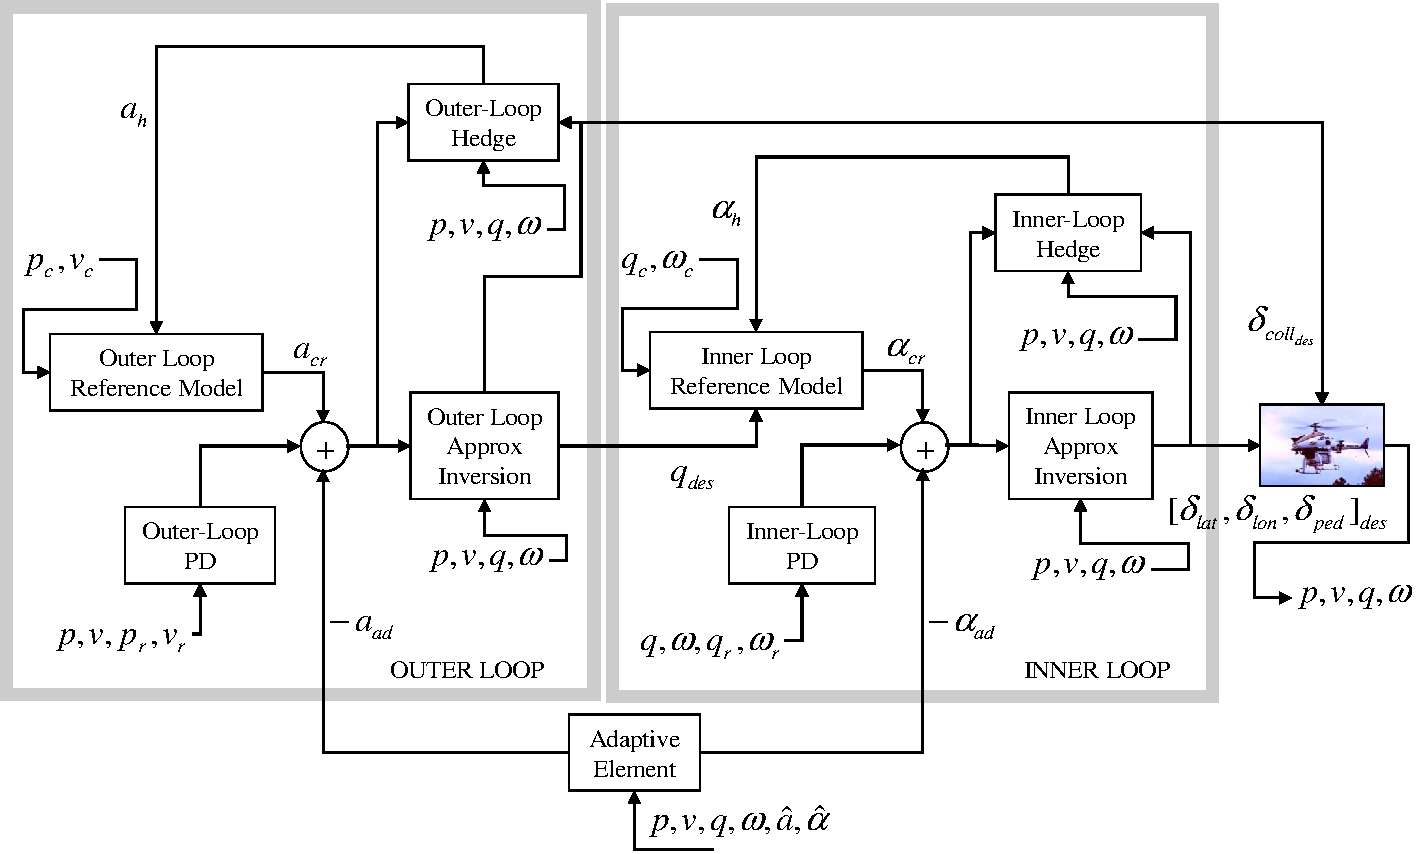
\includegraphics[]{detailarch}
  \centering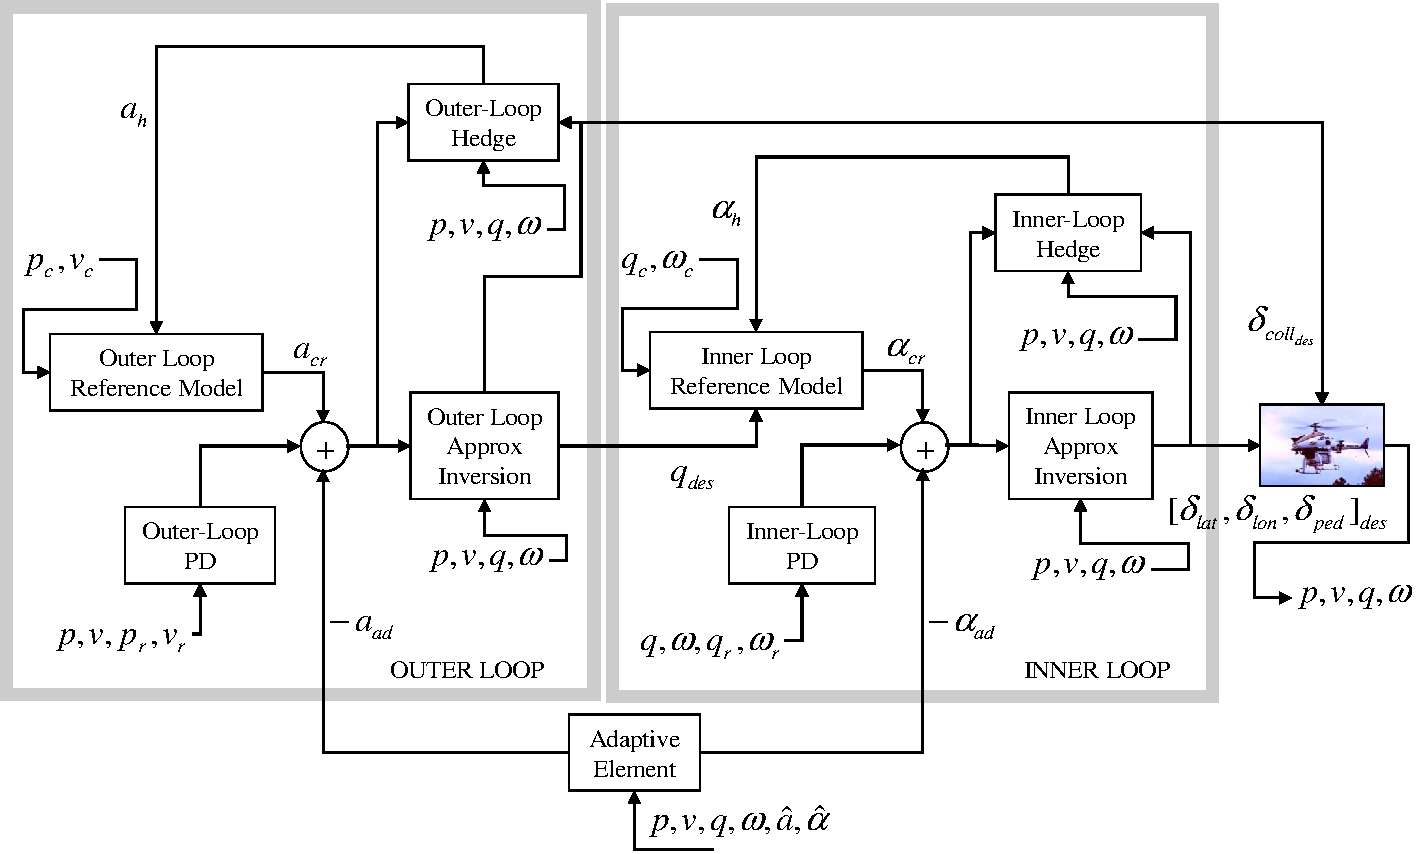
\includegraphics[width=1.4\textwidth,angle=90]{detailarch}
  \caption{Detailed inner and outer loop controller architecture for an autonomous helicopter.}
  \label{f:detailarch}
\end{figure}
Noting that \eq{e:pdot} and \eq{e:quatdot} represent exactly known kinematics, approximate models for translational acceleration, $\ahat$ and a model for angular acceleration, $\alhat$ need to be established.

\[
\begin{bmatrix}
\ades \\
\aldes
\end{bmatrix}
=
\begin{bmatrix}
\ahat (\bfp,\bfv,\qdes,\bfomega,\delfdes,\delhm)\\
\alhat(\bfp,\bfv,\bfq,\bfomega,\delhf,\delmdes)
\end{bmatrix},
\]
Here, $\ades$ and $\aldes$ are commonly referred to as the pseudocontrol
and represent desired accelerations. Additionally, $\delfdes,\delmdes,\qdes$ are the
control inputs and attitude expected to achieve the
desired pseudo-control. This form assumes that translational
dynamics are coupled strongly with attitude dynamics, as is the case
for a helicopter. From the outer-loop's point of view, $\bfq$
(attitude), is like a \emph{virtual actuator} that generates translational
accelerations and $\qdes$ is the desired attitude that the
outer-loop inversion expects will contribute towards achieving the
desired translational acceleration, $\ades$. The dynamics of $\bfq$
appears like actuator dynamics to the outer loop.

\begin{note}
Although the models are approximate, their functional dependence on vehicle rigid body and actuator states are stated accurately for completeness. It is likely that a specific approximate model that is introduced might drop some of this dependency.
\end{note}

\begin{note}
The attitude
quaternion $\qdes$ will be used to augment the externally commanded
attitude $\qc$ to achieve the desired translational accelerations.  Ideally, the trajectory generator would generate a commanded attitude $\qc$ that is consistent with the translational acceleration profile needed to track $\xc(t)$ and $\vc(t)$. If not, the outer-loop inverse takes care of correcting it by an amount necessary to achieve the desired translational accelerations in the longitudinal and lateral directions.
\end{note}

The models have a functional dependence on current actuator position. Because actuator positions are often not measured on small unmanned aerial vehicles, estimates of the actuator positions $\delhm, \delhf$
can be used. When the actuator positions are directly
measured, they may be regarded as known $\delhm = \delm$ and $\delhf
= \delf$. In fact, in the outer loop's case, good estimates of the roll and pitch attitude virtual actuators are
available using inertial sensors and a navigation filter.
%
The approximate models may now be inverted to obtain the desired control and attitude
%
\begin{equation}
\begin{split}
\label{e:inverselaw}
\begin{bmatrix}
\delfdes \\
\qdes
\end{bmatrix}
&=
\begin{bmatrix}
\inv{\ahat_{\delf}}(\bfp,\bfv,\adesdelf,\bfomega,\delhm)\\
\inv{\ahat_{\bfq}}(\bfp,\bfv,\adesq,\bfomega,\delhm)
\end{bmatrix}  \\
\delmdes &= \inv{\alhat}(\bfp,\bfv,\bfq,\bfomega,\delhf,\aldes),
\end{split}
\end{equation}
with $\adesdelf+\adesq = \ades$, $\ahat_{\delf},\ahat_{\bfq}$
formulated to be consistent with \eq{e:inverselaw} and where
actuator estimates are given by actuator models
\begin{equation}\label{e:ghat} \dot{\delh} =
\begin{bmatrix}
\delhfd \\
\delhmd
\end{bmatrix}
=
\begin{bmatrix}
\hat{\bfg}_f(\bfx,\delhf,\delfdes)\\
\hat{\bfg}_m(\bfx,\delhm,\delmdes)
\end{bmatrix}
= \ghat(x,\delh,\deldes).
\end{equation}
%

%In later sections, it will be shown that $\alhat$, can just be an
%approximate linear model of vehicle attitude dynamics and $\ahat$ a
%set of simple equations relating translational accelerations to the
%attitude of the vehicle.
%
Introducing the inverse control law \eq{e:inverselaw} into
\eq{e:vdot} and \eq{e:omdot} results in the following closed-loop
translational and attitude dynamics
%
\begin{align}\label{e:integrator}
\vd &= \ades  + \Delbar_{a}(\bfx,\bfdelta,\delh) -\ah \nonumber \\
 \od &= \aldes + \Delbar_{\bfalpha}(\bfx,\bfdelta,\delh) - \alh,
\end{align}
%
%
where%
\begin{equation}\label{e:Delbar}
\Delbar(\bfx,\bfdelta,\delh) =
\begin{bmatrix}
\Delbar_{a}(\bfx,\bfdelta,\delh) \\
\Delbar_{\bfalpha}(\bfx,\bfdelta,\delh)
\end{bmatrix}
=
\begin{bmatrix}
\bfa(\bfx,\bfdelta) - \ahat(\bfx,\delh) \\
\bfalpha(\bfx,\bfdelta) - \alhat(\bfx,\delh)
\end{bmatrix},
\end{equation}
are static nonlinear functions (model error) that arise due to
imperfect model inversion and errors in the actuator model $\ghat$. The main discrepancy between $g(\cdot)$ and $\ghat(\cdot)$ is the lack of a magnitude saturation function in $\ghat$. This is required in order to maintain invertibility.
The signals, $\ah$ and $\alh$, represent the pseudocontrol that
\emph{cannot be achieved} due to actuator input characteristics such as
saturation. If the model inversion were perfect and no magnitude-saturation
were to occur, $\Delbar,\ah$ and $\alh$ would vanish leaving only
the pseudocontrols $\ades$ and $\aldes$.

Two tasks now remain, (1) Stabilize the feedback linearized dynamics and (2) Address the effects of model error.
The desired accelerations may be designed as
%
\begin{equation}
\begin{split}\label{e:nu}
\ades  &= \acrm  + \apd  - \ahad \\
\aldes &= \alcrm + \alpd - \alhad,
\end{split}
\end{equation}
%
where $\acrm$ and $\alcrm$ are outputs of reference models for the
translational and attitude dynamics respectively. $\apd$ and $\alpd$
are outputs of proportional-derivative (PD) compensators; and
finally, $\ahad$ and $\alhad$ are the outputs of an adaptive element designed to cancel model error $\Delbar$. The effects of
input dynamics, represented by $\ah,\alh$ will first be addressed in
the following section by designing the reference model dynamics such
that they do not appear in the tracking error dynamics. The
reference model, tracking error dynamics, and boundedness are
discussed in the following sections with details of the adaptive element left to \appdx{s:network}.
%
\subsection{Reference Model and Hedging}
Any dynamics and nonlinearities associated with the actuators $\delm,
\delf$ have not yet been considered in the design. If they become
saturated (position or rate), the reference models will continue to
demand tracking as though full authority were still available.
Furthermore, the inner loop appears like an actuator with dynamics to
the outer loop. Practical operational limits on the maximum attitude
of the aircraft may have also been imposed in the inner-loop
reference model. This implies that the outer-loop desired attitude
augmentation $\qdes$ may not actually be achievable, or at the very
least is subject to the inner-loop dynamics.

If the reference model is designed as
\begin{equation}
\begin{split}
\label{e:rmnopch}
\vd_{r} &= \acrm (\prm,\vrm,\pc,\vc) \\
\od_{r} &= \alcrm(\qrm,\orm,\qc\oplus\qdes,\oc),
\end{split}
\end{equation}
where $\prm$ and $\vrm$ are the outer-loop reference model states
and $\qrm$, $\orm$, are the inner-loop reference model states.
The external command signal is $\bfx_c =
\begin{bmatrix}\pc^T & \vc^T & \qc^T & \oc^T\end{bmatrix}^T$. The attitude rotation desired by the outer loop is now added to the
commands for the inner loop controller. Here, $\qc \oplus \qdes$
denotes quaternion multiplication\cite{stevens2003} and effectively concatenates the two rotations.

If tracking error dynamics is computed by subtracting \eq{e:nu} from \eq{e:rmnopch}, the un-achievable acceleration $\ah, \alh$ will appear in the tracking error dynamics. When an adaptive element such as a neural network or integrator is introduced, these effects of input dynamics propagate into the training signal and eventually result in the adaptive element attempting to correct for them leading to incorrect adaptation.

Tackling this issue involves redesigning the reference model by subtracting the deficit accelerations (pseudo-control hedging)
\begin{align}
\label{e:pddrm}
\vd_{r} &= \acrm (\prm,\vrm,\pc,\vc) - \ah \\
\label{e:qddrm} \od_{r} &= \alcrm(\qrm,\orm,\qc\oplus\qdes,\oc) -
\alh,
\end{align}
$\ah$ and $\alh$ are the differences between commanded pseudocontrol
and an estimate of the achieved pseudocontrol. It is an estimate because actual actuator positions may not be known. Additionally, the aircraft state vector $\bfp,\bfv,\bfq,\bfomega$ are estimated using a Kalman Filter~\cite{henrik:jacic:2006,chowdhary:gnc11:2011}. However, for purposes of control design, they are assumed to be known and thus the virtual actuators such as attitude may be assumed to be known in the PCH computation. This assumption may have to be revisited in the case where the control/observer pair is not assumed to be separable, perhaps in a tough localization problem where the control inputs directly affect the observability of the aircraft states.

The PCH signals are given by
%
\begin{align} \label{e:ah}
\ah   &= \ahat (\bfp,\bfv,\qdes,\bfomega,\delfdes,\delhm) - \ahat(\bfp,\bfv,\bfq,\bfomega,\delhf,\delhm) \nonumber \\
      &= \ades                                - \ahat(\bfp,\bfv,\bfq,\bfomega,\delhf,\delhm)\\
\label{e:alh}
\alh  &= \alhat(\bfp,\bfv,\bfq,\bfomega,\delhf,\delmdes) - \alhat(\bfp,\bfv,\bfq,\bfomega,\delhf,\delhm)\nonumber\\
      &= \aldes                   -
      \alhat(\bfp,\bfv,\bfq,\bfomega,\delhf,\delhm).
\end{align}
%
The hedge signals $\ah$, $\alh$, do not directly affect
the reference model output $\acrm$, $\alcrm$, but do so only
through subsequent changes in the reference model states.

The command tracking error may now be defined as $\bfer$
\begin{equation}
\label{e:er} \bfer \triangleq
\begin{bmatrix}
\pc - \prm \\
\vc - \vrm \\
\tilde{Q}(\qc,\qrm) \\
\oc - \orm
\end{bmatrix},
\end{equation}
with corresponding command tracking error dynamics given by
\begin{equation}
\label{e:edotr} \dot{\bfer} =
\begin{bmatrix}
\vc - \vrm \\
\ac - (\acrm - \ah) \\
\oc - \orm \\
\alc - (\alcrm - \alh)
\end{bmatrix},
\end{equation}
The particular form of the reference model dynamics chosen for the translational dynamics, $\acrm$, and attitude dynamics, $\alcrm$, has profound effects on the overall response and controllability of the system. This is fully expounded in Chapter 4 of \cite{kannan:phd} and in \cite{kannan:cdc:2010b}. Also see \cite{kannan:acc:2003} for a discussion on the effects of reference model poles when various elements saturate.

\begin{comment}
A summary of the options for reference models is given here. A definition is useful at this point.
\begin{definition}
\label{def:nullcontstate} A state $x_0$ is said to be null
controllable in time $T
> 0$ if there exists an admissible control $\delta(t)$ such that the state
trajectory $x(t)$ of the system satisfies $x(0) = x_0$ and $x(T) =
0$. The set of all states that are null controllable in time $T$,
denoted by $\mathcal{C}(T)$, is called the null controllable region
in time $T$. The set of all such $x_0$ for $T\in[0,\infty]$ is call the null controllable region.
\end{definition}

Determining the null controllable region of a system is not trivial.
For linear systems, simple estimates may be found using the Circle
and Popov criteria as described in \cite{khalil:book:1992,pittet:cdc:1997}.
Less conservative estimates may be found as the result of an LMI
optimization as described in \cite{hu:book:2001}. For nonlinear systems of
the form \sys{e:simple:fxu}, there is no known method \cite{sontag:siam:1988,sontag:cdc:1988} to explicitly characterize a null controllable region
$\nulldom{x}$ where there always exists an admissible control which
can bring an initial state $x(0)$ back to the origin in finite time.
\end{comment}

As a summary, three reference models were considered.
\begin{itemize}
\item A \emph{Linear Reference Model} will attempt to elicit a linear response in the plant when no such response is possible (peaking) as the plant is nonlinear, especially with the magnitude saturation of actuators.
\item The \emph{Nested Saturation-based Reference Model} is an alternative to the linear reference model containing saturations functions appearing in a nested form and is based on the work by Teel\cite{teel:scl:1997,teel:itac:1996}. This form allows one to restrict the evolution of states in a prescribable manner.
\item The \emph{Constrained Linear Reference Model} is a special case of the nested saturation-based reference model, that is locally linear near the origin.
\end{itemize}

For the quadratic candidate Lyapunov functions chosen in \cite{kannan:phd}, only the nested-saturation and constrained linear reference models have their Lyapunov derivative bounds on the PCH signals $\ah,\alh$. In this chapter the constrained reference model is used with equations given later in \secti{s:helirefmodel}.

\begin{comment}
\begin{equation}
\label{e:refmodelgains}
\begin{bmatrix}
\apd \\
\alpd
\end{bmatrix} =
\begin{bmatrix}
R_p & R_d & 0   &   0 \\
0   & 0   & K_p &   K_d
\end{bmatrix}\bfe,
\end{equation}
\end{comment}


%
\subsection{Tracking error dynamics}
\label{s:trackingerrordynamics} The tracking error
vector is defined as, $\bfe$, as
\begin{equation}
\label{e:e} \bfe \triangleq
\begin{bmatrix}
\prm - \bfp \\
\vrm - \bfv \\
\tilde{Q}(\qrm,\bfq) \\
\orm - \bfomega
\end{bmatrix},
\end{equation}
%
where, $\tilde{Q}:\real{4}\times\real{4} \mapsto \real{3}$, is a
function~\cite{ejohnson:phd} that, given two quaternions results
in an error angle vector with three components. An expression for
$\tilde{\bm{Q}}$ is given by
%
\begin{align}
\label{e:quaterr}
\tilde{Q}(\bfp,\bfq) &= 2sgn(q_1p_1 + q_2p_2 + q_3p_3 + q_4p_4) \times \nonumber \\
&\qquad
\begin{bmatrix}
-q_1p_2 + q_2p_1 + q_3p_4 - q_4p_3 \\
-q_1p_3 - q_2p_4 + q_3p_1 + q_4p_2 \\
-q_1p_4 + q_2p_3 - q_3p_2 + q_4p_1
\end{bmatrix}.
\end{align}
%
The output of the PD compensators may be written as
%
\begin{equation}
\label{e:pdgains}
\begin{bmatrix}
\apd \\
\alpd
\end{bmatrix} =
\begin{bmatrix}
R_p & R_d & 0   &   0 \\
0   & 0   & K_p &   K_d
\end{bmatrix}\bfe,
\end{equation}
%
where, $R_p,R_d \in \real{3\times3}$, $K_p,K_d \in \real{3\times3}$
are linear gain positive definite matrices whose choice is discussed
below. The tracking error dynamics may be found by directly
differentiating \eq{e:e}
%
\[
\dot{\bfe} =
\begin{bmatrix}
\vrm - \bfv \\
\vd_{r} - \vd \\
\orm - \bfomega \\
\od_{r} - \od
\end{bmatrix}.
\]
%
Considering $\dot{\bfe}_2$,
%
\[
\begin{split}
\dot{\bfe}_2 &= \vd_{r} - \vd \\
          &= \acrm - \ah - \bfa(\bfx,\bfdelta) \\
          &= \acrm -\ades + \ahat(\bfx,\delh) - \bfa(\bfx,\bfdelta) \\
          &= \acrm -\apd -\acrm + \ahad + \ahat(\bfx,\delh) - \bfa(\bfx,\bfdelta)\\
          &= -\apd - (\bfa(\bfx,\bfdelta) - \ahat(\bfx,\delh) - \ahad) \\
          &= -\apd - (\Delbar_a(\bfx,\bfdelta,\delh) - \ahad), \\
\end{split}
\]
%
$\dot{\bfe}_4$ may be found similarly. Then, the overall tracking
error dynamics may now be expressed as
%
\begin{equation}\label{e:edot}
\dot{\bfe} = A\bfe + B\left[ \nuhad -
\Delbar(\bfx,\bfdelta,\delh)\right],
\end{equation} where, $\Delbar$ is given by \eq{e:Delbar},
\begin{equation}
 \nuhad = \begin{bmatrix}\ahad \\ \alhad
\end{bmatrix},
\label{e:AB} A =
\begin{bmatrix}
0     &    I     &    0    &   0 \\
-R_p  &   -R_d   &    0    &   0 \\
0     &    0     &    0    &   I \\
0     &    0     &   -K_p  & -K_d
\end{bmatrix},
B =
\begin{bmatrix}
0   &   0 \\
I   &   0 \\
0   &   0 \\
0   &   I
\end{bmatrix}.
\end{equation}
%
and so the linear gain matrices must be chosen such that $A$ is
Hurwitz. Now, $\nuhad$ remains to be designed in order to cancel
the effect of $\Delbar$.


Note that commands, $\delmdes,\delfdes,\qdes$, do not appear in
the tracking error dynamics. PCH allows adaptation to continue when
the actual control signal has been replaced by any arbitrary signal
and thus allows switching between manual and automatic flight during
flight tests without any transients. Furthermore, if the actuator is considered ideal and the actual
position and the commanded position are equal, addition of the PCH
signal $\ah$, $\alh$ has no effect on any system signal.

%
The adaptive signal $\nuhad$ contains two terms
\[
\nuhad = \nuad + \nur = \begin{bmatrix} \aad + \bfa_r \\
\alad + \bfalpha_r\end{bmatrix},
\]
where $\nuad$ is the output of the Single Hidden Layer (SHL) Neural Network (NN) described in
\secti{s:network}. For an air vehicle with adaptation in all degrees
of freedom, $\nuad \in \real{6}$, where the first three outputs,
$\aad$, approximates $\Del_a$ and the last three outputs, $\alad$,
approximate $\Del_{\alpha}$ and is consistent with the definition of
the error in \eq{e:e}.  The term, $\nur\ = [\bfa_r^T, \bfalpha^T_r]^T
\in \real{6}$ is a robustifying signal that arises in the proofs of
boundedness found in \cite{kannan:phd}.



\subsection{Boundedness}
Noting that the plant states are given by
\begin{equation}
\label{e:nrm:plantstates} \bfx(t) = \bfx_r(t) - \bfe(t),
\end{equation}
boundedness of the reference model states $\bfx_r(t)$ is sufficient to establish boundedness of the plant states $\bfx(t)$. However, the reference model dynamics now includes the PCH signal which could be arbitrary and large. The problem of actuator saturation has effectively been moved from affecting the tracking error dynamics to affecting the command-tracking error dynamics of the reference model. If boundedness of \sys{e:edotr} can be established then an assumption that the external command $\xc(t)$ is bounded is sufficient to establish boundedness of the overall system.
%It can be shown that if the tracking error dynamics \sys{e:edot}, which includes the adaptive element can be shown to be bounded,
The following assumptions are required to guarantee boundedness
%\begin{enumerate}
%\item The external command $\bfx_c$ is bounded,$\left\| \bfx_c \right\| \leq \bar{x}_c$.
%\item The SHL NN adaptive element's approximation of $\Del(x,\delh) = \nuad(x,\delh) + \epsilon$ holds in a compact
\begin{assumption}
\label{ass:kcascade:CommandBounded} The external command $\bfx_c$ is
bounded,
\begin{equation*}
\left\| \bfx_c \right\| \leq \bar{x}_c.
\end{equation*}
\end{assumption}

\begin{assumption}
\label{ass:kcascade:NetworkApproxHolds} The NN approximation
$\Del(x,\delh) = \nuad(x,\delh) + \epsilon$ holds in a compact
domain $\domd$, which is large enough such that
$\dom{x_c}\times\dom{e_r}\times\dom{e}\times\dom{\Zt}$ maps into
$\domd$. This assumption is required to leverage the universal approximation property of SHL NN \cite{hornik:itnn:1989}.

%for the error vector defined as
%\[
%\eta = \begin{bmatrix}e \\ vec(\Vt) \\ vec(\Wt) \end{bmatrix}
%\]
%and the compact set containing the origin
%\[
%B_r = \left\{\eta\quad:\quad \| \eta \| \leq r \right\}
%\]
%and for and if $\eta \in B_r$, then $x$ remains in $\domd$.
\end{assumption}
%
\begin{assumption}
\label{ass:kcascade:IdealWeightsBounded}The norm of the ideal
weights $(V^*,W^*)$ is bounded by a known positive value,
\begin{equation*}
0 < \left\|Z^*\right\|_F \leq \bar{Z},
\end{equation*}
where $\|\cdot\|_F$ denotes the Frobenius norm. This is justified due to the universal approximation property of SHL NN if the previous assumption holds \cite{hornik:itnn:1989}.
\end{assumption}
%
\begin{assumption}
\label{ass:kcascade:FixedPoint}Note that, $\Del$ depends on $\nuad$
through the pseudocontrol $\nu$, whereas $\nuhad$ has to be designed
to cancel $\Del$. Hence the existence and uniqueness of a
fixed-point-solution for $\nuad = \Del(\bfx,\nuad)$ is assumed.
Sufficient conditions\cite{calise:automatica:2001} for this assumption are
also available.
\end{assumption}

\begin{assumption}
\label{ass:kcascade:nullRegion} Noting that the null controllable region of the plant $\nulldom{x}$ is not
necessarily a connected or closed set, assume that $\domd \subseteq
\nulldom{x}$, and that $\domd$ in addition to being compact is also
convex.
%there exists a convex compact set $\dom{x} \subset \nulldom{x}$,
%such that $\dom{x_c}\times\dom{e_r}\times\dom{e}\times\dom{\Zt}$
%maps into $\dom{x}$.
%
%such that $\xc \in \dom{x}$ and the trajectory of the reference
%model is such that $x_r(t) - e(t) \in \dom{x} \forall t> 0$.
\end{assumption}


The adaptive element training signal, $r$, adaptive element output, $\nuad$, and robustifying
term, $\nur$, are given by
\[
\begin{split}
r      &= (e^TPB)^T \\
\nuhad &= \nuad + \nur \\
\nuad  &= W^T\sigma(V^T\xbar) \\
\nur   &= -K_r(\|Z\|_F + \bar{Z})r\frac{\|e\|}{\|r\|}.
\end{split}
\]

\begin{theorem}
\label{t:boundedness}
Consider the system
given by (\ref{e:pdot},\ref{e:vdot},\ref{e:quatdot},\ref{e:omdot}), with the inverse law
\sys{e:inverselaw}, reference models (\ref{e:acrm},\ref{e:alcrm}) which
is consistent with (\ref{e:pddrm},\ref{e:qddrm}),  where the gains are
the same as those selected such that the system matrix in
\sys{e:edot} is Hurwitz and assumptions (\ref{ass:kcascade:CommandBounded},\ref{ass:kcascade:NetworkApproxHolds},\ref{ass:kcascade:IdealWeightsBounded},\ref{ass:kcascade:FixedPoint},\ref{ass:kcascade:nullRegion}) are met. If $K_r > 0 \in \real{k\times k}$ is chosen sufficiently large with
lower-limit stated in the proof, and adaptive element weights $W, V$ satisfy the
adaptation laws
\begin{equation}
\label{e:shladaptivelaws}
\begin{split}
\dot{W} &= -\left[ (\sigma - \sigma' V^T \xbar ) r^T + \kappa \|e\| W \right]\Gamma_W \\
\dot{V} &= -\Gamma_V \left[ \xbar (r^T W^T \sigma' )+ \kappa\|e\| V
\right],
\end{split}
\end{equation}
with, $\Gamma_W, \Gamma_V > 0$, $\kappa > 0$ with lower-limit stated
in the proof, and the external command $x_c(t)$ is such that $e_r(t)
\in \lvl(P_r,\rho)$, for some $\rho
> 0$, then, the command tracking error, $\bfer$, the reference model
tracking error, $\bfe$, and adaptive element weights ($\Wt,\Vt$) are uniformly
ultimately bounded. Further, the plant states, $x$, are ultimately
bounded.
\end{theorem}
\begin{proof}
See proof of Theorem 4 in \cite{kannan:phd}.
\end{proof}
\begin{note}
The update laws $\dot{W}(t), \dot{V}(t)$, closely resembles the backpropagation method of tuning neural network weights \cite{Rumelhart:86Nature,Suykens:96bk,Haykin:98bk,Kim:98bk}. However, it is important to note that the training signal $r$ is different from that of the backpropagation based learning laws.
\end{note}


